\tocsection{\textbf{10/15/26 Lecture 15:} Hierarchical Models and Markov Chain Monte Carlo}

\begin{example}{\textbf{Example:} Batting Averages}
    Suppose we want to predict a batter's ``true'' batting average from $n_i$ at-bats. Suppose $X_i \given \theta_i \overset{\tt{ind}}{\sim} \Binom(n_i, \theta_i)$. We want to shrink $\theta_i$ to more reasonable values based on historical data, so say that typically,
    \[ \theta_i \given \alpha, \beta \iidsim \tt{Beta}(\alpha, \beta) \]
    Now, if we don't know $\alpha$ and $\beta$, we can assume $\alpha, \beta \sim \lambda$ and learn $\alpha$ and $\beta$ from prior data. For a particular $\alpha, \beta$, the posterior mean is $\frac{X_i + \alpha}{n_i + \alpha + \beta}$, so when $\alpha, \beta$ are not known, we will consider the posterior mean
    \[ \bb{E}\left[\frac{X_i + \alpha}{n_i + \alpha + \beta} \given X\right] \]
\end{example}

\begin{example}{\textbf{Example:} Gaussian Hierarchical Models}
    Let $\tau^2 \sim \lambda_0$, $\theta_i \given \tau^2 \iidsim N(0, \tau^2)$, and $X_i \given \theta, \tau^2 \overset{\tt{ind}}{\sim} N(\theta_i, 1)$ for $i \leq d$.

    Then, the posterior mean is
    \begin{align*}
        \delta_i(X) &= \bb{E}[\theta_i \given X]\\
        &= \bb{E}\left[\bb{E}[\theta_i \given X, \tau^2] \given X\right]\\
        &= \bb{E}\left[\frac{\tau^2}{1 + \tau^2}X_i \given X\right]\\
        &= \bb{E}\left[\frac{\tau^2}{1 + \tau^2} \given X\right]X_i
    \end{align*}
    where $\bb{E}\left[\frac{\tau^2}{1 + \tau^2} \given X\right]$ is the \emph{shrinkage factor}.\\

    Consider $X_i \iidsim N(0, 1 + \tau^2)$. Then,
    \[ \frac{1}{d}\norm{X}^2 \sim \frac{1 + \tau^2}{d}\chi_d^2 \sim \left(1 + \tau^2, \frac{2(1 + \tau^2)^2}{d}\right) \]
    where the notation $(a, b)$ means a distribution with mean $a$ and variance $b$.\\

    Let $\zeta(\tau^2) = \frac{1}{1 + \tau^2}$, so $\delta_i(X) = (1 - \bb{E}[\zeta \given X]) \cdot X_i$. We can see $X_i \sim N(0, \zeta^{-1})$. Now, say that
    \[ \zeta \sim \frac{1}{s^2}\chi_k^2 = \tt{Gamma}\left(\frac{k}{2}, \frac{2}{s^2}\right) \propto \frac{(s^2)^{k/2}}{\Gamma(k/2)}\zeta^{k/2 - 1}e^{-s^2\zeta/2} \]
    and
    \[ X \given \zeta \sim N_d\left(0, \frac{1}{\zeta}I_d\right) \propto_{\zeta} \zeta^{d/2}e^{-\zeta\norm{X}^2/2} \]
    Multiplying the prior times the likelihood to get the posterior,
    \begin{align*}
        \lambda(\zeta \given X) &\propto_{\zeta} \zeta^{(k + d)/2 - 1}e^{-(s^2 + \norm{X}^2) \cdot \zeta/2}\\
        &\propto_{\zeta} \tt{Gamma}\left(\frac{k + d}{2}, \frac{2}{s^2 + \norm{X}^2}\right)\\
        &= \frac{1}{s^2 + \norm{X}^2}\chi_{k + d}^2
    \end{align*}
    This is like adding pseudo-data: we add more degrees of freedom and scale the variance.\\

    The prior expectation is $\frac{k}{s^2}$, and the posterior expectation is $\frac{k + d}{s^2 + \norm{X}^2}$, so
    \[ \delta(X) = \left(1 - \frac{k + d}{s^2 + \norm{X}^2}\right)X_i \]
\end{example}

\textbf{Graphical Idea:}
\begin{center}
    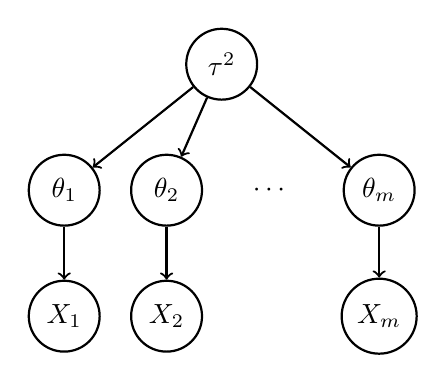
\begin{tikzpicture}[node distance = 1.6cm, every node/.style = {circle, draw, thick, minimum size = 0.9cm}]
        \node (tau) at (0, 0) {$\tau^2$};
        \node (t1) at (-2, -1.6) {$\theta_1$};
        \node (t2) at (-0.7, -1.6) {$\theta_2$};
        \node[draw = none] at (0.6, -1.6) {$\cdots$};
        \node (tm) at (2, -1.6) {$\theta_m$};
        \node (x1) at (-2, -3.2) {$X_1$};
        \node (x2) at (-0.7, -3.2) {$X_2$};
        \node (xm) at (2, -3.2) {$X_m$};
        \draw[->, thick] (tau) -- (t1);
        \draw[->, thick] (tau) -- (t2);
        \draw[->, thick] (tau) -- (tm);
        \draw[->, thick] (t1) -- (x1);
        \draw[->, thick] (t2) -- (x2);
        \draw[->, thick] (tm) -- (xm);
    \end{tikzpicture}
\end{center}
Heuristically,
\begin{enumerate}
    \item Generate $\tau^2$.
    \item Generate $\theta_1, \ldots, \theta_m$ (independently).
    \item Generate $X_1, \ldots, X_m$ (independently).
\end{enumerate}

In general, suppose we have a DAG $(V, E)$ with $V = \{1, \ldots, \abs{V}\}$. Then, if each vertex is a random variable $Z_1, \ldots, Z_{\abs{V}}$, then
\[ p(z_1, \ldots, z_{\abs{V}}) = \prod_{i = 1}^{\abs{V}} p(z_i \given z_{\tt{Pa}(i)}) \]
where $Pa(i) = \{j \col j \to i\}$ is the set of parents of $i$. Then, in our case,
\[ p(\tau^2, \theta_1, \ldots, \theta_m, X_1, \ldots, X_m) = p(\tau^2)\prod_{i = 1}^{m} p(\theta_i \given \tau^2)p(x_i \given \theta_i) \]

\subsection*{Markov Chain Monte Carlo}
\sectionspace

Recall that
\[ \lambda(\theta \given x) = \frac{p_{\theta}(x)\lambda(\theta)}{\int_{\Theta} p_{\zeta}(x)\lambda(\zeta)d\zeta} \]
The numerator is nice, but the denominator is often intractable.\\

\textbf{Computational Strategy:} Set up a Markov chain with stationary distribution proportional to $p_{\theta}(x)\lambda(\theta)$, and run it to get approximate samples.

\begin{definition}[\textbf{Definition 15.1:} Stationary Markov Chains]
    A \emph{stationary Markov chain} with transition kernel $Q(y \given x)$ and initial distribution $\pi_0(x)$ is a sequence of random variables $X^{(0)}, X^{(1)}, X^{(2)}, \ldots$ where $X^{(0)} \sim \pi_0$ and
    \[ X^{(t)} \given X^{(0)}, \ldots, X^{(t - 1)} \sim Q(\cdot \given X^{(t - 1)}) \]
    so $Q(y \given x) = \bb{P}(X^{(t)} = y \given X^{(t - 1)} = x)$.
\end{definition}

\textbf{Note:} A Markov chain is an example of a graphical model:
\begin{center}
    \begin{tikzcd}
        X^{(0)} \arrow[r] & X^{(1)} \arrow[r] & \cdots
    \end{tikzcd}
\end{center}
We see that
\[ \pi_1(y) = p(X^{(1)} = y) = \int_{\cal{X}} Q(y \given x)\pi_0(x)d\mu(x) \]
where $Q(y \given x)\pi_0(x)$ is the probability that we start at $x$ and move to $y$.

\begin{definition}[\textbf{Definition 15.2:} Stationary Distributions]
    We say $\pi$ is a \emph{stationary distribution}, or is \emph{stationary for $Q$}, if
    \[ \pi(y) = \int_{\cal{X}} Q(y \given x)\pi(x)d\mu(x) \]
    That is, if we start in $\pi$, we stay in $\pi$.
\end{definition}

\begin{definition}[\textbf{Definition 15.3:} Detailed Balance]
    We say $\pi$ has \emph{detailed balance} if
    \[ \pi(x)Q(y \given x) = \pi(y)Q(x \given y) \]
    for all $x, y$. That is, $P(\tt{start at } x \tt{ and flow to } y) = P(\tt{start at } y \tt{ and flow to } x)$. If we have detailed balance, we call the chain \emph{reversible}:
    \begin{center}
        \begin{tikzcd}
            X^{(0)} \arrow[r] & X^{(1)}
        \end{tikzcd}
        $\overset{d}{=}$
        \begin{tikzcd}
            X^{(0)} & X^{(1)} \arrow[l]
        \end{tikzcd}
    \end{center}
\end{definition}

\begin{lemma}[\textbf{Lemma 15.4}]
    If $\pi$ has detailed balance, then $\pi$ is stationary.
\end{lemma}
\begin{proof}{Proof:}
    We see that
    \[ \int_{\cal{X}} Q(y \given x)\pi(x)d\mu(x) = \int_{\cal{X}} \pi(y)Q(x \given y)d\mu(x) = \pi(y)\int_{\cal{X}} Q(x \given y)d\mu(x) = \pi(y) \]
    as $\int_{\cal{X}} Q(x \given y)d\mu(x) = 1$.

    $\qed$
\end{proof}

\textbf{Note:} Markov chains are forgetful, as the distribution of $X^{(t)}$ only depends on $X^{(t - 1)}$.

\begin{theorem}[\textbf{Theorem 15.5} Markov Chain Convergence Theorem]
    Suppose a Markov chain with stationary distribution $\pi$ is
    \begin{enumerate}
        \item \textbf{Irreducible:} For all $x, y$, there exists $n$ such that $p(X^{(n)} = y \given X^{(0)} = x) > 0$ (for continuous state spaces, we consider neighborhoods of $y$).
        \item \textbf{Aperiodic:} For all $x$, $\gcd\{n > 0 \col p(X^{(n)} = x \given X^{(0)} = x) > 0\} = 1$.
    \end{enumerate}
    Then, $\tt{Dist}(X^{(t)}) \xrightarrow{t \to \infty} \pi$ (in total variation distance) regardless of $\pi_0$.
\end{theorem}

Letting our stationary distribution be $\pi$ and running the Markov chain, we can approximate properties of its distribution. This method is called \emph{Markov Chain Monte Carlo} (MCMC).

\subsection*{Gibbs Sampler}
\sectionspace

Suppose we have a parameter vector $(\theta_1, \ldots, \theta_d)$.\\

\textbf{Gibbs Sampler Algorithm:}
\begin{center}
    \begin{minipage}{0.6\linewidth}
        Initialize $\theta = \theta^{(0)} \sim \pi_0$\\
        For $t = 1, \ldots, T$:\\
        \hspace*{0.6cm}For $j = 1, \ldots, d$:\\
        \hspace*{1.2cm}Sample $\theta_j \sim \lambda(\theta_j \given \theta_{-j}, X)$ \hfill $(*)$\\
        \hspace*{0.6cm}Record $\theta^{(t)} = \theta$
    \end{minipage}
\end{center}
Here, $\theta_{-j}$ denotes all coordinates but $\theta_j$, and $(*)$ updates the coordinates in the order $1 \to 2 \to \cdots \to d$. Instead of $(*)$, we could alternatively
\begin{enumerate}[label = \alph*)]
    \item Update $1$ random coordinate.
    \item Update all coordinates in a random order.
\end{enumerate}



